\section{Performance Degradation Detection}

% \begin{frame}
%     \vfill
%     \centering
%     \begin{beamercolorbox}[sep=8pt,center,shadow=true,rounded=true]{title}
%     \usebeamerfont{title}\insertsectionhead\par%
%     \end{beamercolorbox}
%     \vfill
% \end{frame}

\begin{frame}
    \frametitle{Why yet another performance degradation detection algorithm}
    \begin{itemize}
        \item \textbf{Imbalanced}: For example, 83.5\% of the 16,868 HSPAP measurements for ISP Mobilis are from one user. If those measurements are excluded, the median RTT can decrease from 332ms to 219ms.
        \begin{itemize}
            \item normal association rules method bias to the performance of the dominating user.
        \end{itemize}
        \item \textbf{Sparse}: Although the total number of observations is huge, records for each combination of features can be very small.
        \begin{itemize}
            \item impossible to model the normal performance for all combinations of features separately.
        \end{itemize}
        \item \textbf{Large}: We need a scalable method to process the increasingly large data.
    \end{itemize}
\end{frame}

\begin{frame}
    \frametitle{Our Method}
    \begin{enumerate}
        \item Find feature sets with enough records using the Apriori algorithm.
        \item Filter the candidate feature set using using some huristic rules.
        \item Identify performance degradation events by comparing the meadian RTT of similar feature sets.
        \item Use hypothesis test to verify influence of the anormaly feature we found.
    \end{enumerate}
\end{frame}

% \begin{frame}
%     \frametitle{Implementation Details}
%
% \end{frame}

\begin{frame}
    \frametitle{Evaluation}
    \begin{enumerate}
        \item Low false positive rate in random data
        \begin{itemize}
            \item We randomly shuffle the RTT of the records.
            \item We mathmatically proved that the probability of our methods flagging an anomaly is very small in our configuration.
        \end{itemize}
    \end{enumerate}
\end{frame}

\begin{frame}
    \frametitle{Evaluation}
    \begin{enumerate}
        % \item Low false positive rate in random data
        \setcounter{enumi}{1}
        \item Real world case of Google Germany
    \end{enumerate}
    \vskip 1em
    \centering
    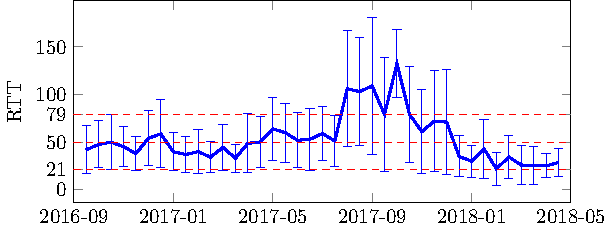
\includegraphics[width=.65\textwidth]{fig/case1.pdf}
\end{frame}

\begin{frame}
    \frametitle{Evaluation}
    \begin{enumerate}
        % \item Low false positive rate in random data
        % \item Real world case of Google Germany
        \setcounter{enumi}{2}
        \item Real world case of Microsoft Office Mobile
    \end{enumerate}
    \vskip 1em
    \centering
    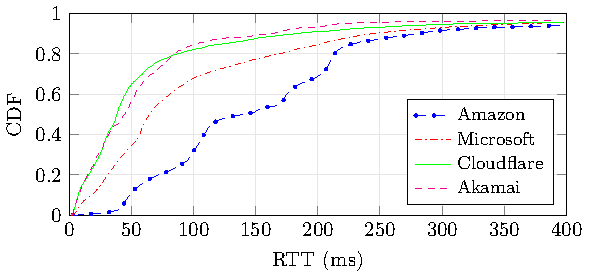
\includegraphics[width=.65\textwidth]{fig/case2.pdf}
\end{frame}
